% Boxology preprint — revision 3 (18 September 2026): TODOs of rev. 2 closed
% Changes from v1 are marked in the accompanying notes; TODO markers flag
% material that must be filled in or implemented before submission.
\documentclass[11pt]{article}
\usepackage[margin=1in]{geometry}
\usepackage{amsmath,amssymb,amsthm}
\usepackage{graphicx}
\usepackage{booktabs}
\usepackage{natbib}
\usepackage[hidelinks]{hyperref}

\graphicspath{{figs/}}

\newtheorem*{model}{Model}
\newtheorem*{identity}{Identity}

% Long file names and URLs in the availability section: let TeX stretch the
% line rather than run it off the page.
\emergencystretch=3em

% Visible placeholder — remove every one of these before submission.
\newcommand{\todo}[1]{\textbf{[TODO: #1]}}

\newcommand{\hPa}{\ensuremath{\,\mathrm{hPa}}}
\newcommand{\dam}{\ensuremath{\,\mathrm{dam}}}
\newcommand{\km}{\ensuremath{\,\mathrm{km}}}
\newcommand{\Kday}{\ensuremath{\,\mathrm{K\,d^{-1}}}}

\title{Boxology: the isobar--thickness box count as an exact advection integral, and its rendering}

\author{Evan J. Lane\\[3pt]
\small ORCID: 0009-0001-7841-6087\\
\small Independent Researcher, Atlanta, Georgia, USA\\
\small 6842 METOC Operational Forecaster, United States Marine Corps (2010--2014)\\
\small FrostByte project\\
\small \texttt{usmclane92@gmail.com} (corresponding author)}
\date{}

\begin{document}
\maketitle

\noindent\emph{This is a non-peer-reviewed preprint submitted to EarthArXiv. Version 2, September 2026. Licensed CC BY 4.0.}

\begin{abstract}
\noindent
``Boxology'' is the hand-analysis practice of reading thermal advection from the angle at which mean-sea-level-pressure isobars cross 1000--500\hPa\ thickness contours: steep crossings cut the chart into small quadrilaterals and imply strong advection, while parallel families imply none. This note shows the practice is an identity within geostrophic balance rather than a rule of thumb, and implements it as a rendered chart product. Splitting the layer-mean geostrophic wind into its bottom-surface and thermal parts removes the thermal wind exactly, since it blows along the thickness contours, so layer-mean thickness advection reduces to a Jacobian of the two plotted fields. Treating those fields as coordinates makes that Jacobian a change of variables, so the advection integrated over any quadrilateral bounded by consecutive isobars and consecutive thickness lines is a fixed quantum, independent of the box's shape, a specialization of the solenoid count in Bjerknes' circulation theorem. Box area and advection intensity are therefore reciprocal, which is what the eye is measuring. A renderer is described that labels the actual quadrilaterals by band index and fills each flat at its own quantum-over-area rate on a doubling ladder. Constants, smoothing, edge handling, and the limits of the geostrophic premise at low latitude, in strongly curved flow, and over high terrain are documented. Against GFS analyses in 48 runs spanning a year, both hemispheres, land and ocean, the box field correlates at $0.95$ with the model's own full-wind layer-mean thickness advection; about half of that advection, two thirds over the United States, is cancelled adiabatically, so the product is a diagnostic and not a forecast.
\end{abstract}

\noindent\textbf{Keywords:} synoptic analysis; thermal advection; circulation theorem; objective analysis; chart rendering

\section{Introduction}

``Boxology'' is the hand-analysis habit of reading thermal advection off a surface chart by eye: where the isobars cross the thickness (or isotherm) lines at a steep angle, the crossing cuts the plane into small quadrilaterals and the air is turning over fast; where the two families run parallel there are no boxes and nothing is advecting \citep{lackmann2011}. The name is weather-school vernacular, taught to enlisted forecasters in their first weeks; the practice it names is standard. This note derives why the technique is exact within geostrophic balance, not a rule of thumb, and documents a renderer that turns the same habit into a field a chart-production pipeline computes and shades rather than one left to the reader's eye.

None of the physics is new. The solenoid count is \citet{bjerknes1898}; the Jacobian form of advection by a geostrophic flow is standard \citep{holton2013}, and thickness advection read from the surface chart goes back to the development literature \citep{sutcliffe1947,petterssen1956}. What this note adds is narrower. First, the corollary, written out for the pair of fields actually drawn on the surface chart, that every isobar--thickness quadrilateral carries the same advection integral, so that box area alone measures local intensity. Second, a renderer that shades those quadrilaterals rather than a smoothed proxy for them. Third, a statement of where the geostrophic premise fails on a routine chart and how the product is withdrawn there. The counting argument was made redundant, for computation, the day model grids could be evaluated pointwise; it survives because it is the argument the eye is making.

\section{The isobar-parallel wind carries the whole signal}

Split the 1000--500\hPa\ layer-mean geostrophic wind into the bottom-surface geostrophic wind plus half the thermal wind, $\mathbf{V} = \mathbf{V}_0 + \tfrac12 \mathbf{V}_T$. The thermal wind blows along the thickness contours by construction, so $\mathbf{V}_T \cdot \nabla h \equiv 0$ and
\begin{equation}
-\mathbf{V}\cdot\nabla h = -\mathbf{V}_0\cdot\nabla h
\label{eq:split}
\end{equation}
identically. Only the isobar-parallel flow advects thickness, which is why the technique is licensed to ignore everything on the chart except the two contour families it is already reading, and why it is an identity rather than an approximation. The decomposition and (\ref{eq:split}) hold pointwise for variable $f$, since $f$ enters $\mathbf{V}_T$ only as a scalar factor and does not turn it off the thickness lines.

The same cancellation nearly holds at every level between the bounding surfaces. The geostrophic wind at pressure $p$ is $\mathbf{V}_0 + (g/f)\,\hat{\mathbf{k}}\times\nabla h_p$, with $h_p$ the 1000--$p$ thickness, so $\mathbf{V}_g(p)\cdot\nabla h = \mathbf{V}_0\cdot\nabla h$ exactly at 500\hPa, where $h_p = h$, and at 1000\hPa, trivially; in between it fails only by the angle between $\nabla h_p$ and $\nabla h$, which is small wherever the direction of the thermal gradient does not turn much with height. Geostrophic advection of the layer thickness is therefore very nearly level-independent, and comparing (\ref{eq:jac}) against advection of the same thickness field by the \emph{real} wind at each level measures how geostrophic that level's wind is. \S\ref{sec:verify} does that.

\section{The Jacobian form}

Substituting the geostrophic relation $\mathbf{V}_0 = (g/f)\,\hat{\mathbf{k}}\times\nabla Z_0$ (with $Z_0$ the 1000\hPa\ height, i.e.\ the isobars converted to geopotential meters) into (\ref{eq:split}) turns the advection into a Jacobian of the two plotted fields:
\begin{model}[geostrophic thermal advection]
\begin{equation}
A = -\frac{g}{f}\,J(Z_0,h) = -\frac{g}{f}\,|\nabla Z_0|\,|\nabla h|\,\sin\theta,
\qquad
J(Z_0,h) = \frac{\partial Z_0}{\partial x}\frac{\partial h}{\partial y} - \frac{\partial Z_0}{\partial y}\frac{\partial h}{\partial x},
\label{eq:jac}
\end{equation}
\end{model}
\noindent with $\theta$ the angle at which the isobar crosses the thickness line. Parallel contours ($\theta = 0$) give zero; a perpendicular crossing gives the maximum for that pair of gradient magnitudes. Nothing else in the field enters, which is the same claim (\ref{eq:split}) made, now in a form a renderer can evaluate pointwise. Written this way, (\ref{eq:jac}) is the familiar Jacobian form of geostrophic advection with the surface height as the streamfunction; the point of (\ref{eq:split}) is that the surface height is the \emph{right} streamfunction for the layer-mean thickness, not merely a convenient one.

\section{Box counting as a change of variables}

The reason box area is the thing a hand analyst's eye is measuring follows from treating $(Z_0, h)$ as new coordinates over the plane. The Jacobian of that map is exactly $J$ from (\ref{eq:jac}), so $|J|\,dx\,dy = dZ_0\,dh$, and integrating $A$ over one quadrilateral bounded by two consecutive isobars ($\delta Z_0$ apart) and two consecutive thickness lines ($\delta h$ apart) gives
\begin{identity}[one box, one quantum]
\begin{equation}
\iint_{\mathrm{box}} A\,dA = \mp\frac{g}{f}\,\delta Z_0\,\delta h,
\qquad
A_{\mathrm{box}} = \frac{\delta Z_0\,\delta h}{|J|},
\label{eq:quantum}
\end{equation}
\end{identity}
\noindent the same magnitude for every box regardless of its shape. This is a specialization of the solenoid count in Bjerknes' circulation theorem to a pair of level-set families rather than an arbitrary closed curve \citep{bjerknes1898,lackmann2011}: box count carries the area integral of $A$ over a region (Green's theorem reduces it to a signed count around the boundary, $\iint_R A\,dA = -\frac{g}{f}\oint_{\partial R} Z_0\,dh$); box area carries the local intensity, and the two are reciprocal per (\ref{eq:quantum}). That reciprocity is the whole reason the hand technique works by eye, and it is why the renderer described in \S\ref{sec:render} keys its shading intensity to $A$ (equivalently, to $A_{\mathrm{box}}^{-1}$) rather than to any separately-tuned quantity.

Equation (\ref{eq:quantum}) treats $f$ as constant over the box, and the same-quantum statement is therefore exact between boxes at the same latitude. The quantum scales as $1/f = 1/(2\Omega\sin\varphi)$, so an identically spaced box at $30^\circ$N carries about $1.7$ times the integral of one at $60^\circ$N. Within a single box the fractional variation of the quantum is $\cot\varphi\,\Delta y/a$ for a meridional extent $\Delta y$ and Earth radius $a$: under $1\%$ for the $43\km$ boxes at the top of the ladder in \S\ref{sec:render}, and about $8\%$ for the $490\km$ boxes at its floor at $45^\circ$N. The box-rate routine uses the mean of $|f|$ over the cells of each box, so (\ref{eq:quantum}) is applied box by box with its own local quantum; the sign of the box is the sign of the box-mean of the pointwise $A$. The box-mean of $|f|$ differs from $f$ at the centroid only at second order in the box's meridional extent, well inside the variation just quoted. The Green's-theorem count around a large region inherits the same caveat and should be read with $f$ at the region's centroid.

\section{Temperature form}
\label{sec:temp}

The hypsometric relation $h = (R_d/g)\,\bar{T}\ln 2$ for the 1000--500\hPa\ layer converts (\ref{eq:jac}) to the advective contribution to the layer-mean temperature tendency,
\begin{equation}
\frac{\partial \bar{T}}{\partial t} = -\frac{g^2}{f R_d \ln 2}\,J(Z_0,h),
\label{eq:temp}
\end{equation}
returned in $\Kday$. $Z_0$ is recovered from MSLP via the standard $8\,\mathrm{m\,hPa^{-1}}$ conversion ($p \approx 1000 + Z_{1000}/8$), so the overlay reads exactly the field the isobars on the chart were drawn from.

Equation (\ref{eq:temp}) is the advective term only. The ascent that warm advection forces cools the column adiabatically, and on a real grid about half of the advective signal is cancelled that way, two thirds over the continental United States (\S\ref{sec:verify}). The rates on the ladder in \S\ref{sec:render} are advection, not forecast temperature change, and the product is not a forecast.

\begin{center}
\small\begin{tabular}{@{}lp{0.36\textwidth}p{0.36\textwidth}@{}}
\toprule
Quantity & Symbol / value & Note \\
\midrule
Layer coefficient & $g^2/(R_d\ln 2) \approx 0.4833\ \mathrm{K\,s^{-2}}$ & divide by local $f$ for $\mathrm{K\,s^{-1}}$ per unit $J$ \\
MSLP $\to Z_0$ & $8\,\mathrm{m\,hPa^{-1}}$ & $p \approx 1000 + Z_{1000}/8$ \\
Equator fade & $12$--$20^\circ$ & tapered, not cut, to 0 \\
Curvature fade & $\mathrm{Ro} = 1$--$3$ & tapered, not cut, to 0; see \S\ref{sec:limits} \\
Terrain fade & $1000$--$2000$\,m & tapered, not cut, to 0; see \S\ref{sec:limits} \\
House contour intervals & $\delta p = 4\hPa$ ($2\hPa$ on the globe and the trajectory chart), $\delta h = 6\dam$ & box size only; the rate does not depend on them \\
\bottomrule
\end{tabular}
\end{center}

\subsection{Where the geostrophic premise fails}
\label{sec:limits}

Equation (\ref{eq:jac}) inherits every assumption of geostrophic balance, and three regimes on a routine chart fall outside it. Each is tapered smoothly to zero rather than masked at a hard edge, because a hard edge draws a false analysis boundary across the map.

\paragraph{Low latitude.} $f \to 0$ makes (\ref{eq:jac}) blow up, and the geostrophic relation itself stops holding well before the true equator. The field is tapered through $12$--$20^\circ$ latitude.

\paragraph{Strongly curved flow.} In a tropical cyclone, or any tight closed low, the surface flow is in gradient rather than geostrophic balance, and geostrophy overestimates the isobar-parallel wind by a factor that grows with the curvature Rossby number
\begin{equation}
\mathrm{Ro} = \frac{|\mathbf{V}_0|\,|\kappa|}{f} = \frac{g}{f^2}\,|\nabla Z_0|\,|\kappa|,
\qquad
\kappa = \nabla\cdot\!\left(\frac{\nabla Z_0}{|\nabla Z_0|}\right),
\label{eq:ro}
\end{equation}
where $\kappa$ is the curvature of the isobars, computable from the same field as everything else. In gradient balance the cyclonic wind is $|\mathbf{V}_0|\,(\sqrt{1+4\mathrm{Ro}}-1)/(2\mathrm{Ro})$: about $0.75\,|\mathbf{V}_0|$ for $\mathrm{Ro} \approx 0.5$, typical of the center of a mature midlatitude cyclone and smaller still along its frontal zones where the boxes live, but under $0.1\,|\mathbf{V}_0|$ at the $\mathrm{Ro} \gg 10$ a tropical cyclone produces. Since only $\mathbf{V}_0$ enters (\ref{eq:split}), the box rate inherits that overestimate directly, on top of the small-$f$ amplification a tropical system already sits in. An axisymmetric warm core would in fact give $J = 0$, since concentric isobars and thickness lines are parallel, but real cores are sheared off their pressure centers, the two families cross at small angles, and with gradients this steep even small angles pin the ladder. The field was therefore tapered linearly from full weight at $\mathrm{Ro} = 1$ to zero at $\mathrm{Ro} = 3$, with $\mathrm{Ro}$ evaluated from the same smoothed $Z_0$ the isobars are drawn from; where $\nabla Z_0 \to 0$ the curvature is undefined and the weight is left at one, since $J$ vanishes there anyway. That left midlatitude cyclones essentially untouched and removed tropical cyclones and tight thermal lows. There is one taper, not two: the trajectory chart of \S\ref{sec:transport} takes the product of the latitude, curvature, and terrain weights from the same routine as the box field, carries the minimum of that product along each back-trajectory, and hatches wherever the minimum fell below $0.99$. Figures 1--4 were rendered with all three tapers on.

\paragraph{High terrain.} MSLP and the 1000\hPa\ height are extrapolations below ground over most of a continent. That is harmless at a few hundred meters and not at the elevation of the Great Basin or the Colorado Plateau, where a kilometer or more of fictitious column is being assumed and the reduced pressure gradient inherits the terrain's temperature structure. The field is tapered with surface elevation by the same construction as the latitude taper: full weight at or below $1000$\,m, zero at or above $2000$\,m. Elevation is the ETOPO1 ice-surface relief model, not the forecast model's orography and not a bedrock grid, which would put the Antarctic plateau near sea level. The floor is the elevation above which the suite already refuses to plot station sea-level pressure, for the same reason; the ceiling is the floor of the high intermountain basins. No single elevation separates the High Plains east of the Rockies, where post-frontal cold advection is real and matters, from the Great Basin at similar height, so the ramp is a judgment call and it has a cost: the plains between about $1000$ and $1500$\,m keep their boxes at half weight or better, one rung down the ladder at most, while the Great Basin, the Colorado Plateau, the Mexican Plateau, and Tibet go blank. Figure~\ref{fig:conus} shows the same analysis with the taper off and on.

The gradient-wind ratio is deliberately not applied as a correction. It would repair the tropical cyclones and destroy (\ref{eq:quantum}), since the correction varies within a box and the thermal wind no longer drops out cleanly. The identity is kept exact where its premise holds, and the display is withdrawn where it does not.

\section{Rendering: the boxes themselves}
\label{sec:render}

The renderer shades the actual quadrilaterals, not a smooth field standing in for them. A box is one connected region over which both band indices $\lfloor p/\delta p\rfloor$ and $\lfloor h/\delta h\rfloor$ are constant: the pair changes exactly where a contour is drawn, so such a region is the polygon bounded by the four lines around it, and the box-labeling routine recovers every box on the chart without tracing or intersecting a single contour. Connectivity is 4-way, not 8-way: two boxes touching only at a corner meet at an isobar/thickness crossing, which is the one place they are guaranteed to be different boxes, and 8-way connectivity welds them into a blob straddling the very feature being measured.

Each box is then filled flat, at the rate (\ref{eq:quantum}) assigns it: its own quantum over its own area, so a slack box is weak and a tight one intense. The shading routine bins that rate into eight bands, each edge doubling the one below ($3, 6, 12, \ldots, 384\Kday$). Because $A_{\mathrm{box}} \propto A^{-1}$, box side scales as $A^{-1/2}$, so a doubling ladder in $A$ is a $\sqrt{2}$ ladder in box side, roughly $490\km$ at the floor down to a $43\km$ knot at the top, the same visual step at every rung, and fill opacity climbs with it, ending at $0.82$ rather than $1$ so the contours and any underlying field stay legible through the deepest box.

The quantum belongs to a whole box, and the labeling returns regions that are not one: the strip between two isobars inside a thickness plateau, the ring between two closed isobars around a low, a tongue that one thickness line enters and leaves by the same side. None of these is bounded by two isobars and two thickness lines, and none integrates to a quantum; a ring integrates to zero, since $Z_0$ is constant on both of its boundaries in the Green's-theorem form above. A region is therefore treated as a box only if it touches a neighbor one isobar band up, one down, one thickness band up, and one down, read off the labeled mesh's own cell edges. Whole boxes are rated at quantum over area. The remainder are rated at the box-mean of the pointwise $|A|$, which is what quantum over area equals for a whole box (\S\ref{sec:checks}) and is small wherever such regions occur. \S\ref{sec:checks} measures what the rule is worth; without it the concentric rings of a tropical cyclone shade as if they were boxes.

Boxes touching the frame are discarded. Those are cut boxes whose measured area is only the part that fits on the chart, so they would read as far tighter than they are; a hand analyst does not count a box running off the map either.

\subsection{Why not a filled contour of $A$}

Equation (\ref{eq:jac}) is defined pointwise, so a filled contour of it is available and was the first implementation. It renders the same quantity and is not the technique: it smooths across the crossings instead of stopping at them, and at chart scale over the thickness ramp it read as a faint wash rather than as boxes. The per-pixel version survives as a hatched overlay option; the production path draws the discrete boxes.

\subsection{Smoothing}

The advection field is a product of two gradients, so it amplifies grid noise the eye never sees on the chart itself. The defaults match what the isobar and thickness fields are already smoothed to on the chart ($\sigma = 3.0$ on MSLP, thickness pre-smoothed at $\sigma = 1.5$ upstream) so the shading never disagrees with the crossing angle a reader can actually see drawn.

\section{Example output}
\label{sec:examples}

Figures~\ref{fig:conus}--\ref{fig:etjet} show the renderer on archived GFS $0.25^\circ$ analyses, the box shading drawn over the same MSLP isobars and 1000--500\hPa\ thickness contours the technique reads by hand, with the 12-hour trails and bolus counts of \S\ref{sec:transport} over them. All are from 07--09 September 2026. Figures~\ref{fig:conus} and \ref{fig:wpac} are late-summer cases in the Northern Hemisphere; Figure~\ref{fig:winter} is the same hour in the Southern Hemisphere's late winter, where the Southern Ocean cyclones draw the cold- and warm-advection couplets the technique exists to find. Isobars are drawn every $2\hPa$ in Figures~\ref{fig:conus}, \ref{fig:wpac}, and \ref{fig:et}, where the late-summer gradients are slack, and every $4\hPa$ in Figure~\ref{fig:winter}; the rate a box is shaded at does not depend on the choice (\S\ref{sec:checks}). The 300\hPa\ analysis is given as a separate panel or figure rather than overlaid, because the surface chart reads better with the jet known and worse with it drawn on top.

Because the product is zero wherever the flow runs along the thickness lines, it separates systems that are baroclinically active now, which draw a warm/cold couplet, from equivalent-barotropic ones, which draw nothing: tropical cyclones in a near-uniform tropical thickness field, and occluded or cut-off lows whose thermal field has wrapped up concentric with their isobars. That is a statement about current thermal advection, not about a system's structure or history, and it is meaningful only inside the validity envelope of \S\ref{sec:limits}. What the boxes register on a cyclone is thermal asymmetry across it: thickness lines crossing the isobars on one flank and not the other. That is the quantity the cyclone phase space of \citet{hart2003} measures with its parameter $B$, the storm-relative thickness difference between the right and left of the track, and in that sense the box field is a chart-scale proxy for $B$ wherever the geostrophic premise holds. It is not a proxy for core type. Tropical, subtropical, and extratropical cyclones are distinguished in that framework by the sign of the thermal wind through the column, that is, whether the core is warm or cold aloft, and a surface-to-500\hPa\ thickness crossing carries no information about that. A symmetric cold-core low draws nothing, and a warm-core storm sheared off its center draws boxes; neither result classifies the system.

The case in Figures~\ref{fig:wpac} and \ref{fig:et} was chosen in advance as a test of the most useful form of that distinction, extratropical transition: a recurving tropical cyclone should draw nothing until it reaches the baroclinic zone and acquires a thermal asymmetry, at which point the couplet should appear. Tropical Storm Krovanh was south of Japan on 07 September 2026 and forecast to go extratropical near Honshu. It did not. The Japan Meteorological Agency carried it as a tropical storm through 06 September 2100Z, downgraded it to a tropical depression at 07 September 0000Z near $26.0^\circ$N, $132.0^\circ$E, and issued no later position; it was never classified extratropical. The analyses agree: the low filled from 996 to 1006\hPa\ while drifting north to Kyushu, and lost its closed circulation in the frontal zone along southern Japan by 09 September. The sequence is therefore the null case, and the box field reads it as one. At no analysis hour does the depression draw a whole box: it sits in a thickness plateau inside a closed 582\dam\ contour, the isobars and the one thickness line around it are nearly concentric, and the trails into it are withheld for curvature. The couplet that does appear belongs to a different system, a frontal wave that forms on the baroclinic zone at the northeastern end of the depression's trough, closes off east of Honshu by 07 September 1200Z, and deepens to 994\hPa\ by 08 September 0000Z with up to two boluses of warm air arriving ahead of it in twelve hours. A depression that fills in place and a wave that deepens next to it are separated by the two contour families alone, which is the claim of the preceding paragraph; the transition the sequence was set up to show remains to be shown on a storm that makes one.

\begin{figure}[p]
\centering
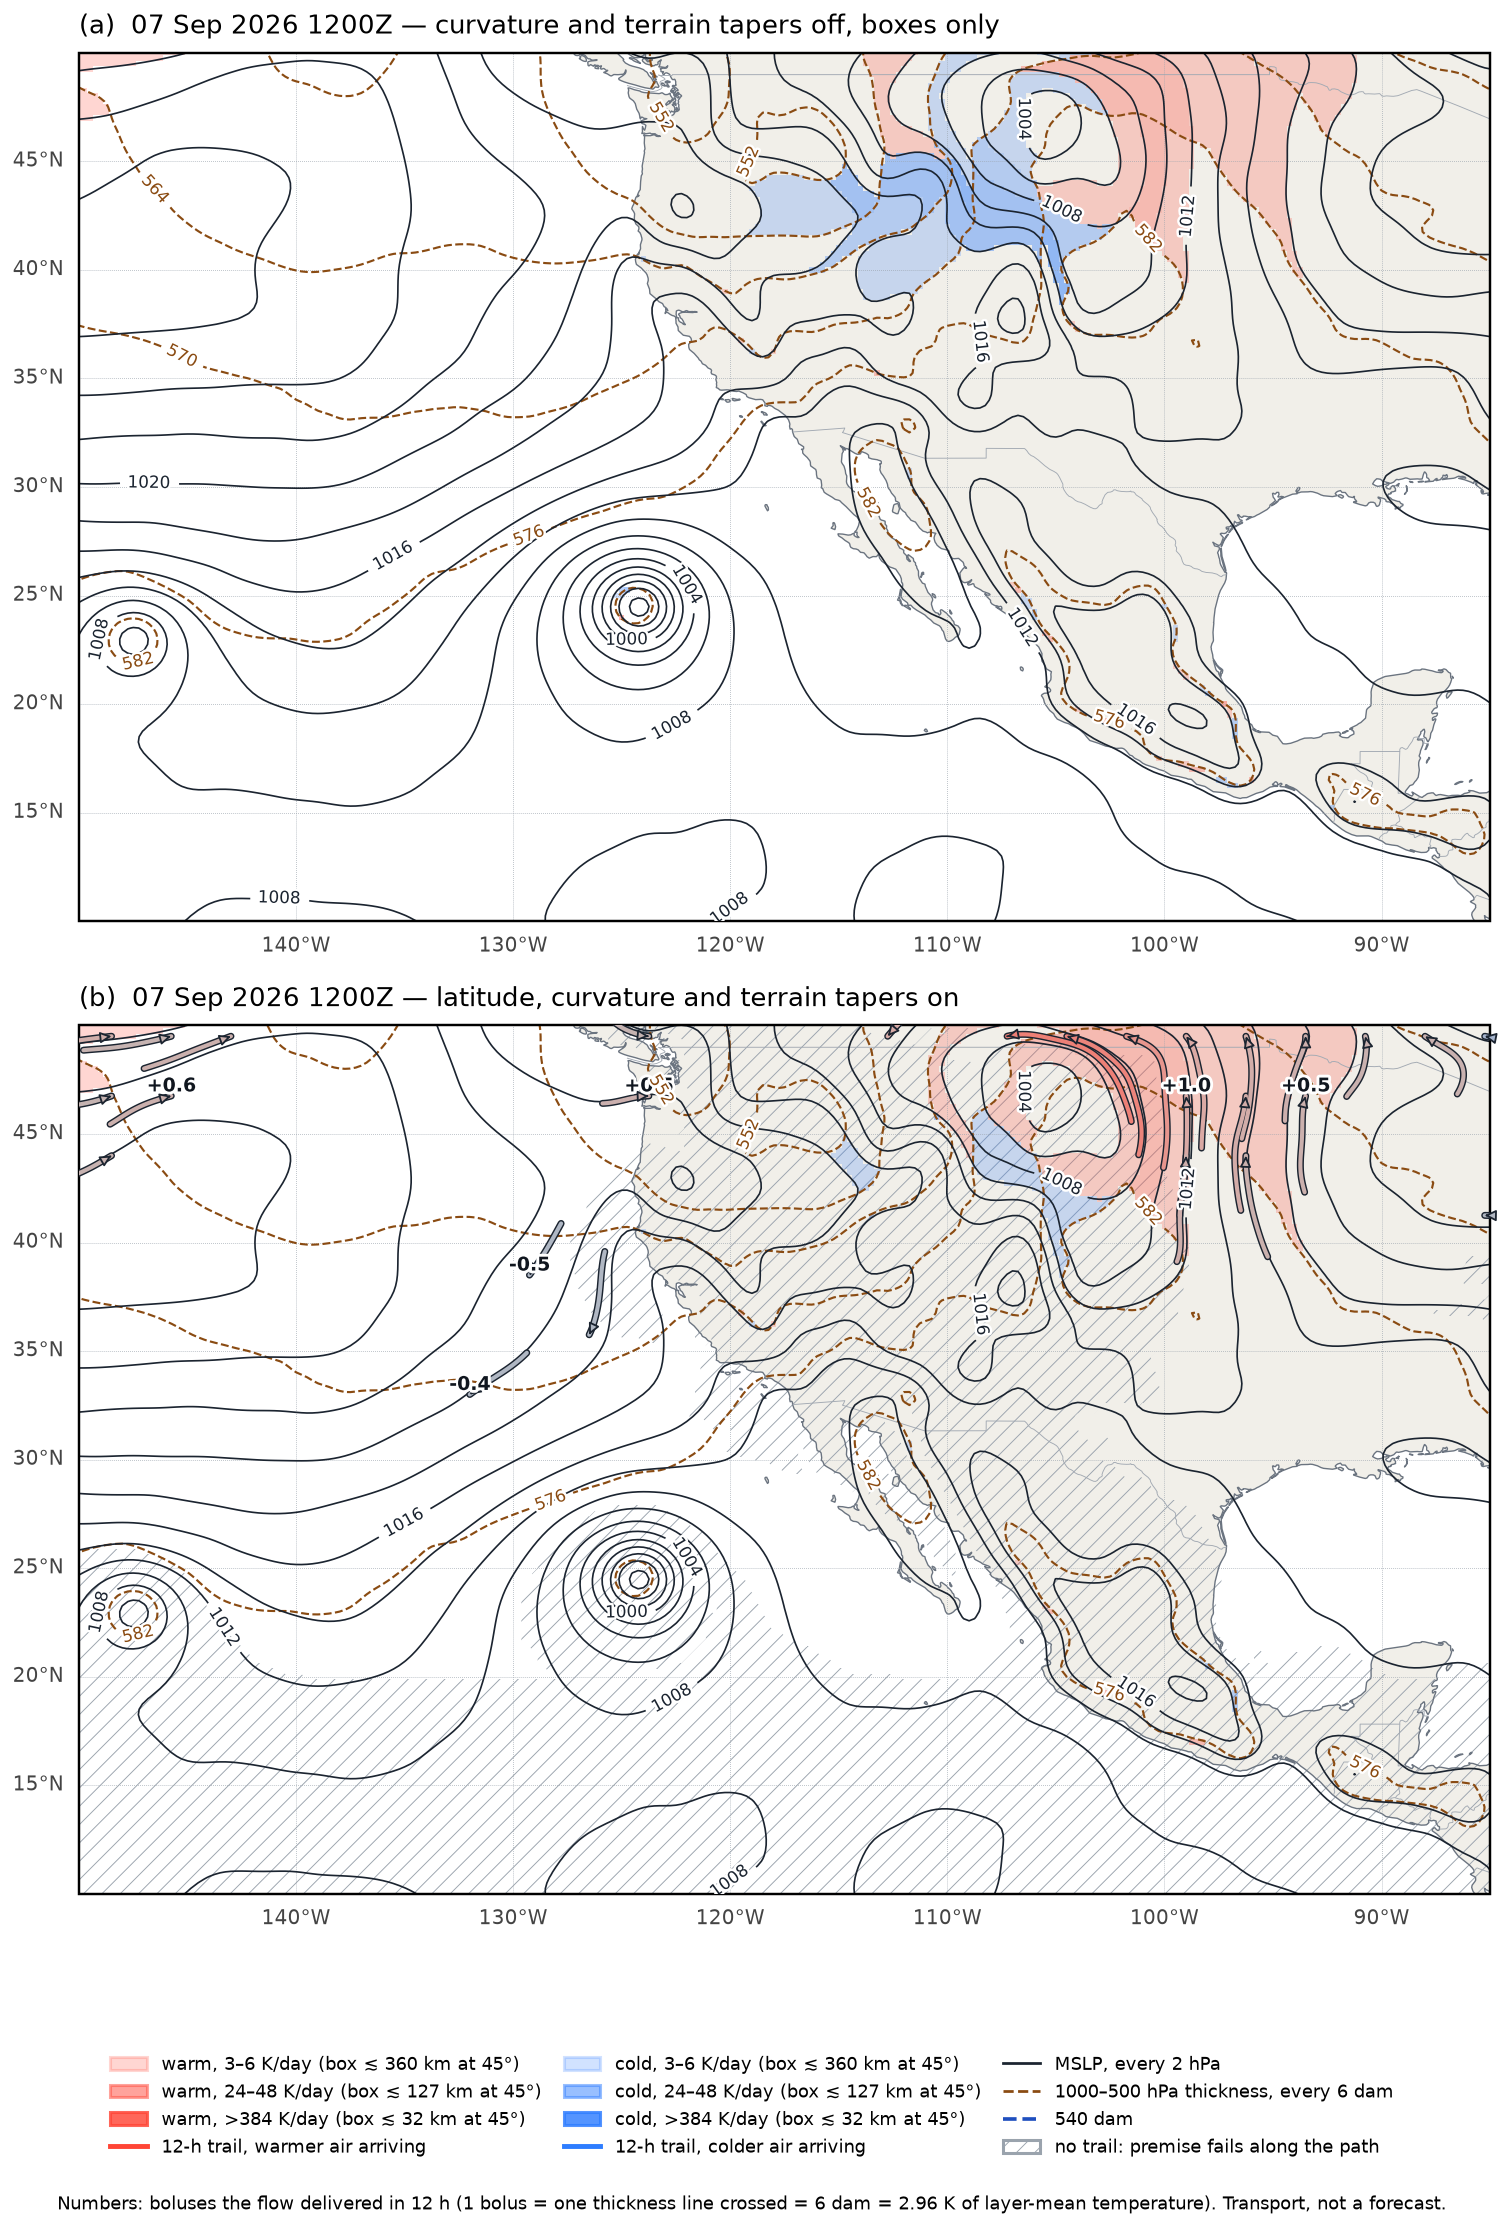
\includegraphics[width=\textwidth,height=0.66\textheight,keepaspectratio]{fig1_conus_sep07.png}
\caption{Western North America and the eastern Pacific, GFS $0.25^\circ$ analysis valid 07 September 2026 1200Z, isobars every $2\hPa$. (a) Boxes only, with the curvature and terrain tapers off (the latitude taper cannot be turned off, since $1/f$ is undefined in the belt). (b) All three tapers on, with the 12-hour trails and their bolus counts; hatching marks ground where no trail is offered because the premise failed somewhere along the back-trajectory. The cold-advection boxes of (a) over the Snake River Plain, the Great Basin, and Wyoming lie on ground between $1300$ and $2200$\,m, where the reduction to 1000\hPa\ is a long extrapolation, and are gone in (b). What survives is the couplet of the 1004\hPa\ low on the Montana--Saskatchewan border: warm advection ahead of it across the Dakotas and Manitoba, with about one bolus delivered in twelve hours, and the part of the cold advection behind it that lies on the plains below $1500$\,m, at reduced weight. The hurricane near $25^\circ$N, $124^\circ$W draws nothing in either panel: its concentric isobars and closed 582\dam\ line bound rings, not boxes (\S\ref{sec:render}), and in (b) its trails are withheld for curvature as well.}
\label{fig:conus}
\end{figure}

\begin{figure}[p]
\centering
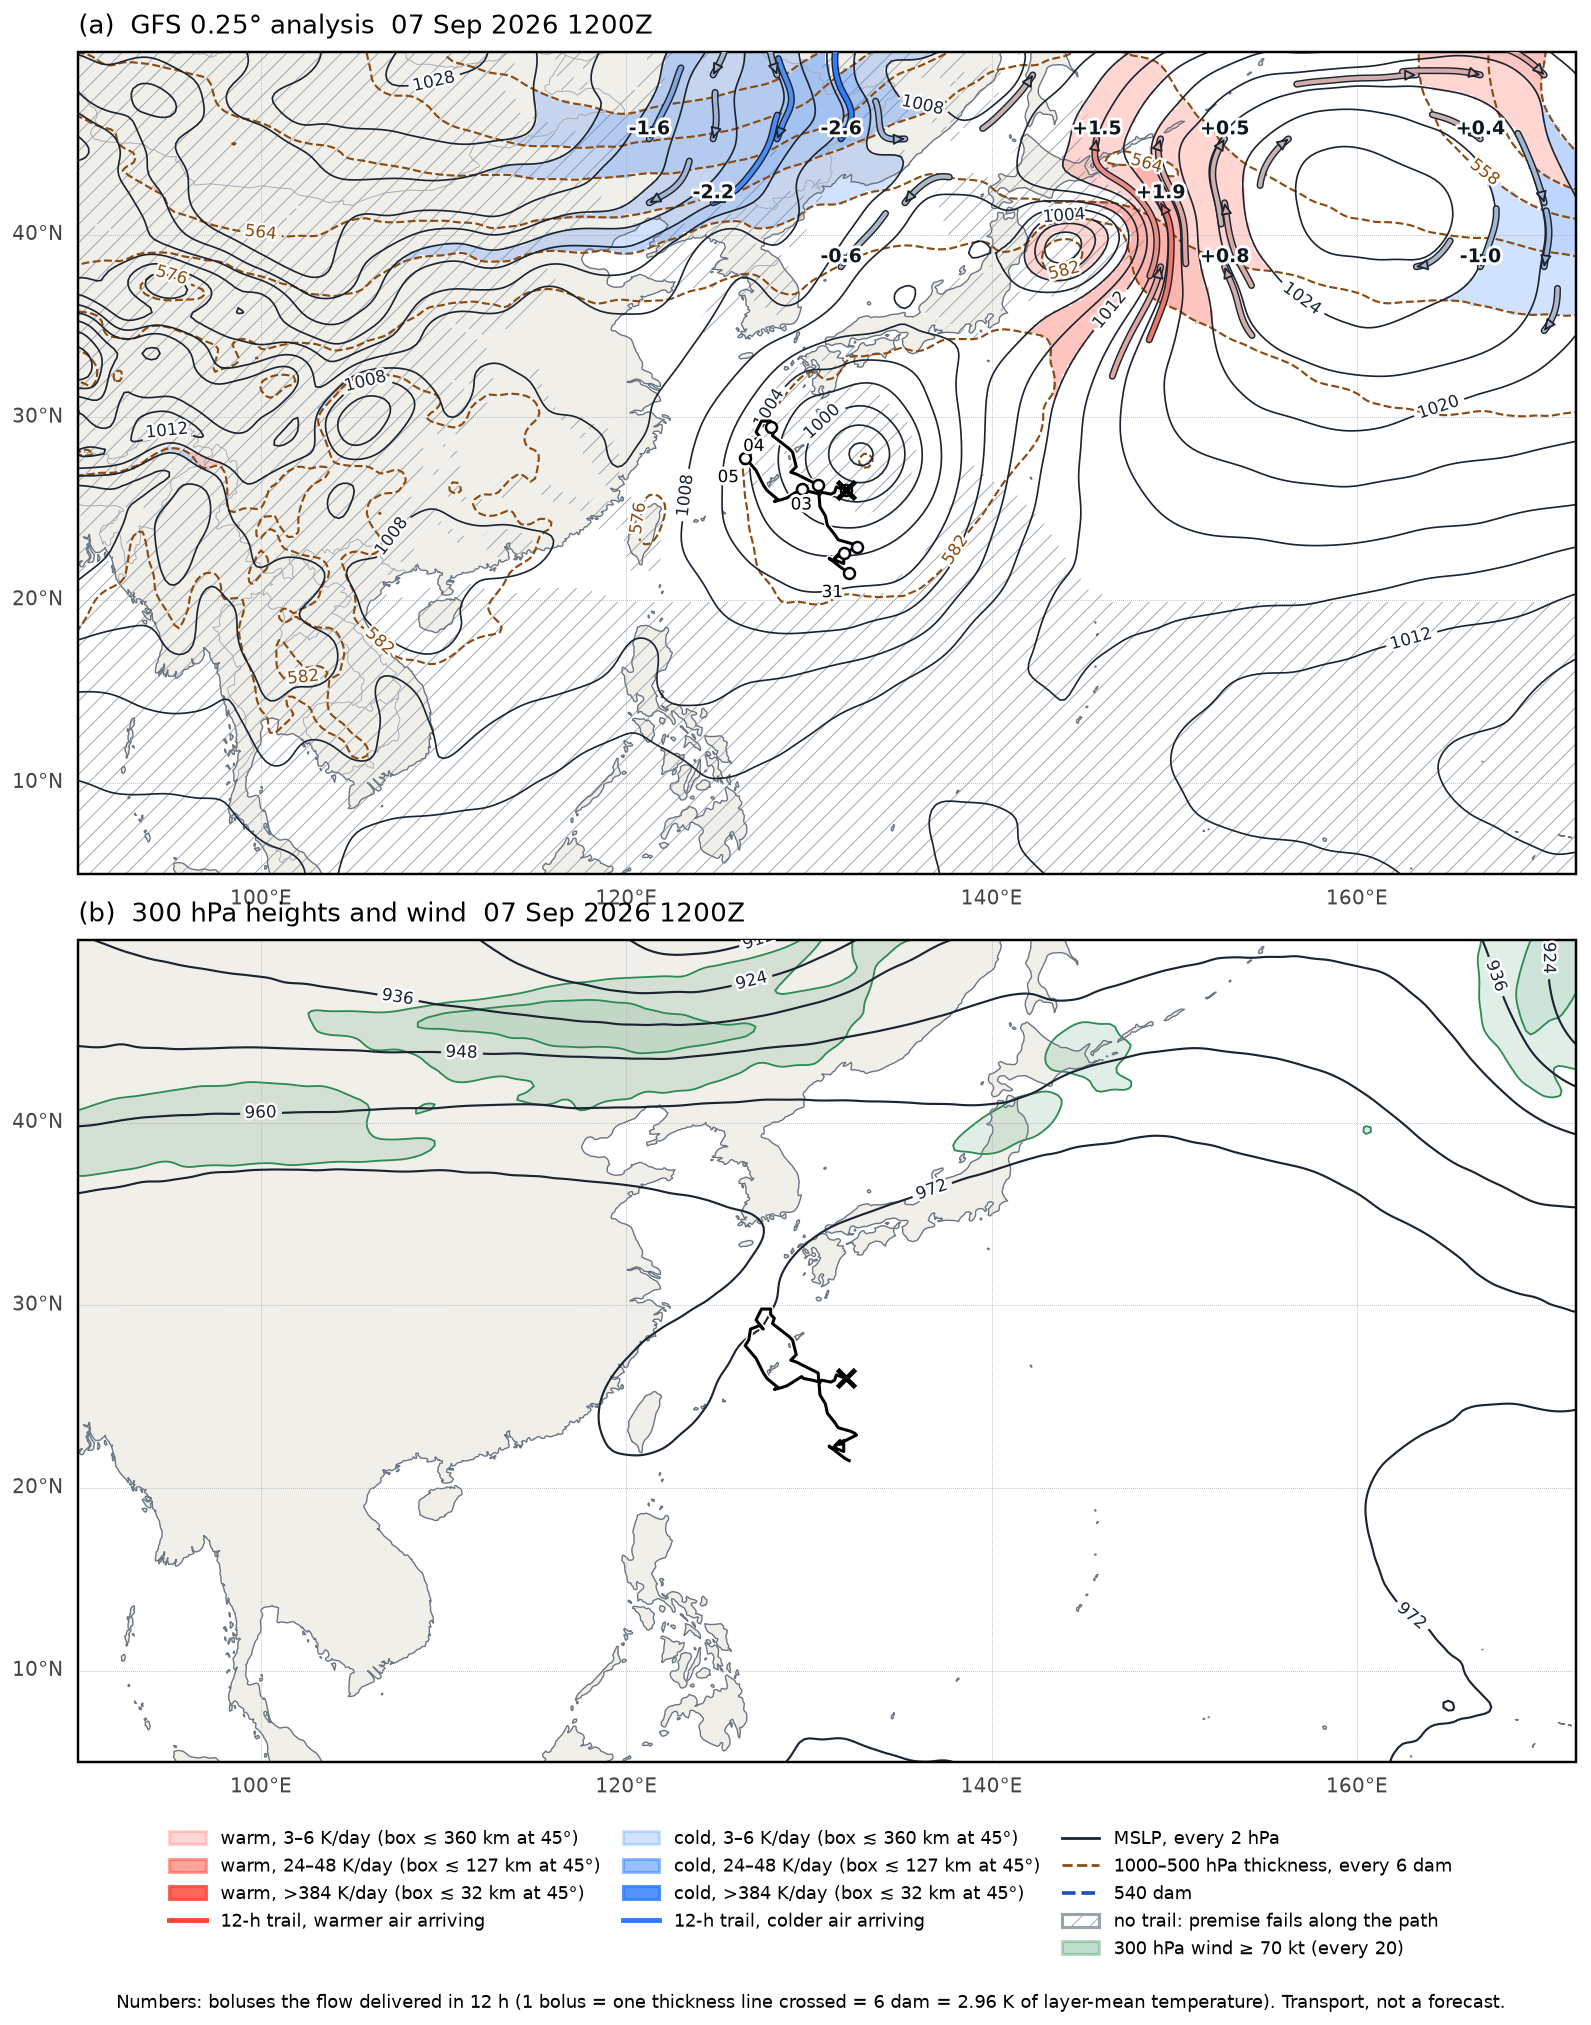
\includegraphics[width=\textwidth,height=0.68\textheight,keepaspectratio]{fig2_wpac_sep07.png}
\caption{East Asia and the western Pacific, GFS $0.25^\circ$ analysis valid 07 September 2026 1200Z. (a) Box field, trails, and bolus counts; the black line is the Japan Meteorological Agency track of Krovanh from 31 August, with a ring at each 0000Z position and a cross at the last one issued, 07 September 0000Z, when the storm was downgraded to a tropical depression. (b) 300\hPa\ heights (every 12\dam) and wind (shaded from 70\,kt, every 20\,kt). The depression, twelve hours after the last advisory position, draws no box and is given no trail. The frontal wave east of Honshu near $39^\circ$N, $144^\circ$E draws the couplet, with up to $1.9$ boluses of warm air delivered ahead of it, beside the only 70\,kt streak near Japan in (b); the polar jet proper is still over Mongolia and northeast China, well north of the depression. The cold-advection band under the trough over northeast China and Korea, $1.6$ to $2.6$ boluses, is inside the premise. Most of China is hatched for terrain and everything south of $20^\circ$N for latitude.}
\label{fig:wpac}
\end{figure}

\begin{figure}[p]
\centering
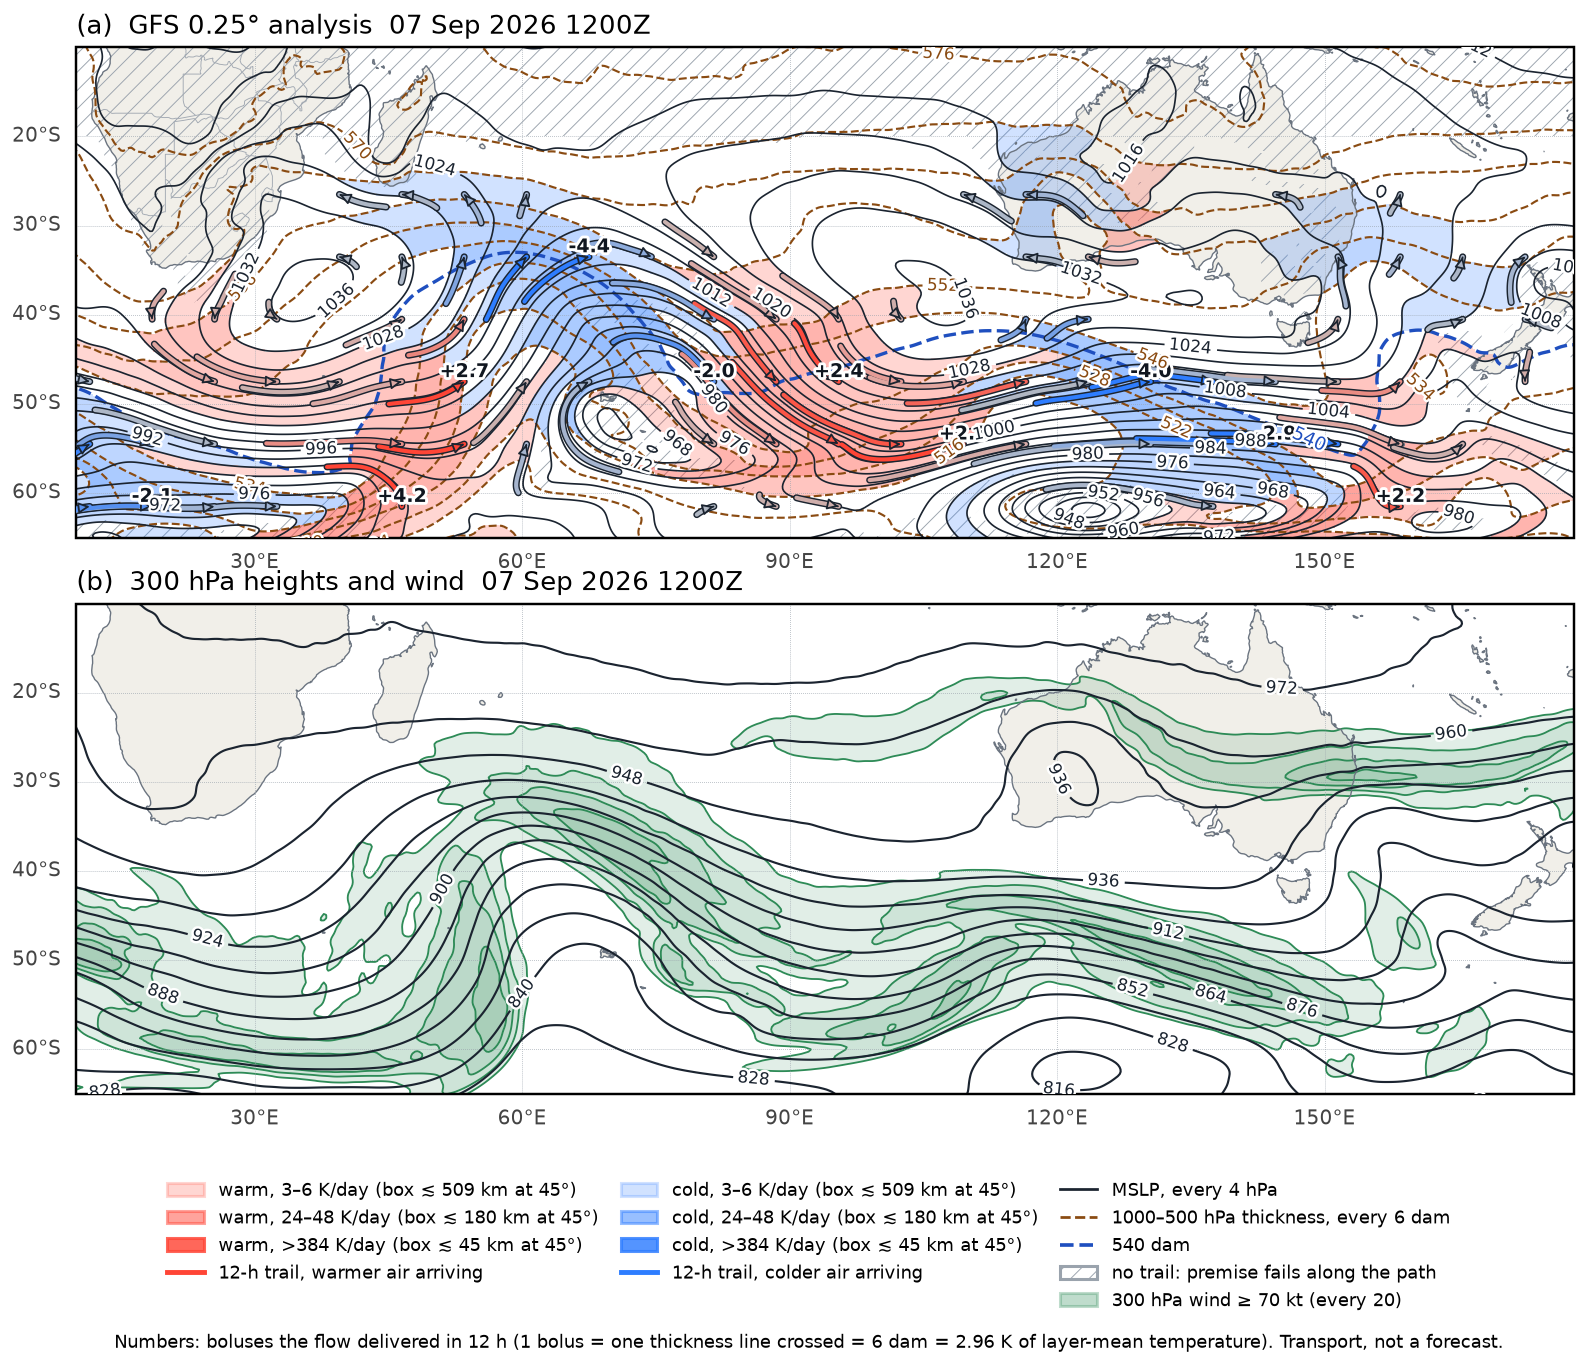
\includegraphics[width=0.92\textwidth]{fig3_sh_sep07.png}
\caption{Southern Hemisphere, Africa to New Zealand, GFS $0.25^\circ$ analysis valid 07 September 2026 1200Z: late winter south of the equator, isobars every $4\hPa$. (a) Box field, trails, and bolus counts. (b) 300\hPa\ heights and wind. The deep cyclones of the Southern Ocean each draw the couplet the technique exists to find: cold-advection boxes on the western flank, where southerlies carry Antarctic air equatorward, and warm-advection boxes ahead, where northerlies push the thickness lines poleward, cold west and warm east, as it must be in this hemisphere. The largest counts on the chart, $-4.4$ boluses near $33^\circ$S, $65^\circ$E and $+4.2$ near $60^\circ$S, $45^\circ$E, both lie along the polar jet in (b). The subtropical ridges draw nothing, and the tropics across the top of the chart are blank under the low-latitude taper. This is the case the consistency checks of \S\ref{sec:checks} were run on.}
\label{fig:winter}
\end{figure}

\begin{figure}[p]
\centering
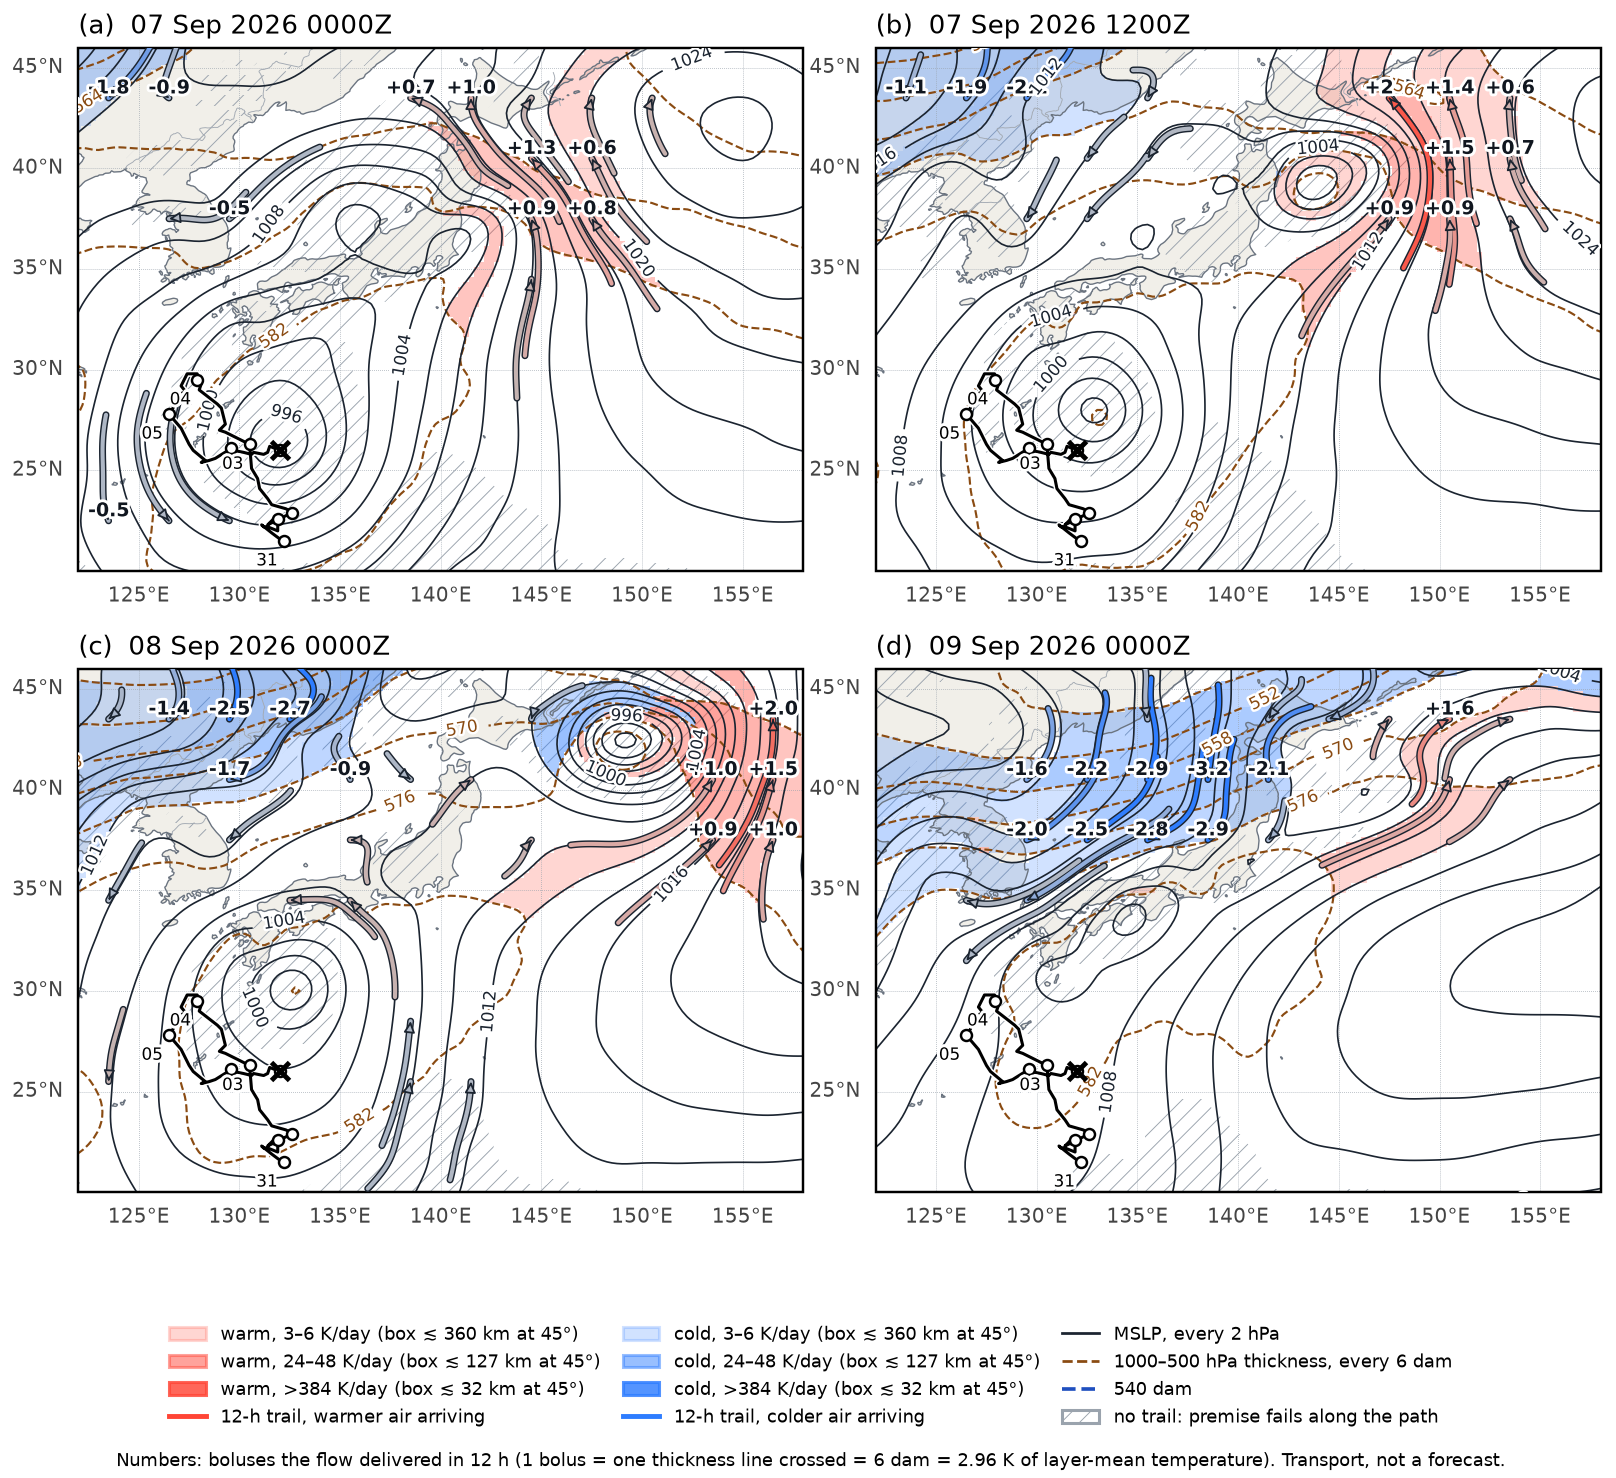
\includegraphics[width=\textwidth]{fig4_krovanh_sequence.png}
\caption{The remnant of Krovanh and the frontal wave beside it: box field, trails, and bolus counts on GFS $0.25^\circ$ analyses at (a) 07 September 2026 0000Z, (b) 1200Z, (c) 08 September 0000Z, and (d) 09 September 0000Z. Figure~\ref{fig:etjet} gives the 300\hPa\ analysis at the same hours. Track and cross as in Figure~\ref{fig:wpac}; positions are from the Japan Meteorological Agency track data as archived by Digital Typhoon (National Institute of Informatics), not from forecast bulletins, and none exists after the cross. (a) At the hour of the downgrade the 996\hPa\ low draws nothing; warm advection, $0.6$ to $1.3$ boluses, lies along the trough running northeast from it across Honshu. (b) The wave has closed off at 1002\hPa\ east of Honshu and draws the couplet. (c) The wave, now 994\hPa\ near $42^\circ$N, $149^\circ$E, has cold advection wrapped behind it and $0.9$ to $2.0$ boluses of warm air arriving ahead; the depression, 1000\hPa\ south of Kyushu, still draws nothing. (d) The depression is an open wave on the front over Kyushu; the boxes on the chart are the post-frontal cold advection over the Sea of Japan and Korea, $1.6$ to $3.2$ boluses.}
\label{fig:et}
\end{figure}

\begin{figure}[p]
\centering
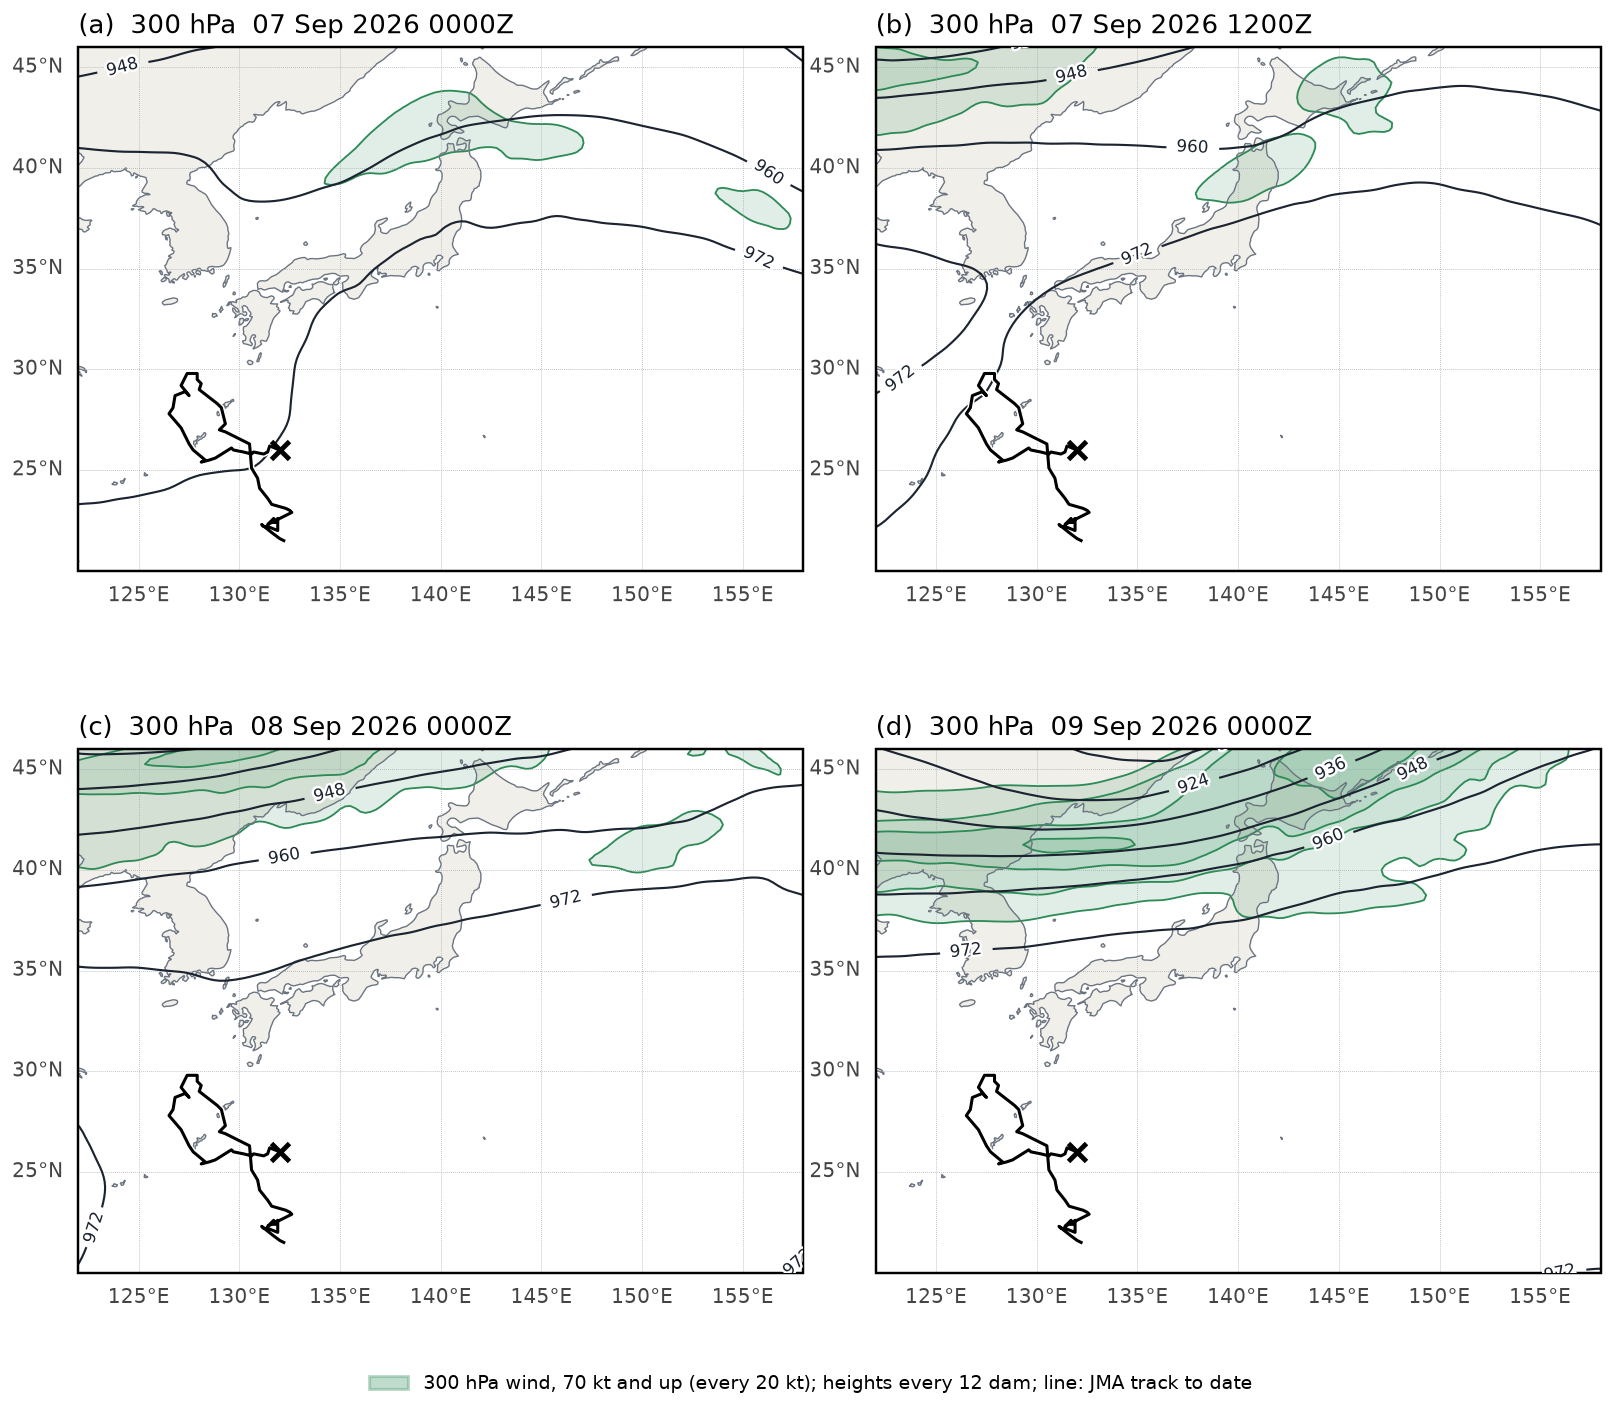
\includegraphics[width=\textwidth]{fig4b_krovanh_300hpa.png}
\caption{300\hPa\ heights (every 12\dam) and wind (shaded from 70\,kt, every 20\,kt) at the four hours of Figure~\ref{fig:et}, with the same track. Through (a)--(c) no 70\,kt wind lies south of $38^\circ$N and the polar jet stays over northeast China; it reaches the Sea of Japan and northern Honshu only in (d), over the post-frontal cold advection and a day after the depression had begun to fill. The depression never came under the jet, which is the upper-air half of why it filled instead of transitioning.}
\label{fig:etjet}
\end{figure}

\section{Transport along the channel}
\label{sec:transport}

Because $\mathbf{V}_0$ runs along the isobars, a parcel carried by it stays in one isobar channel, and its thickness changes by $\delta h$ at every thickness line it crosses. The box count along a channel is therefore the thickness change the geostrophic flow delivers to that parcel: the Lagrangian counterpart of (\ref{eq:quantum}), which counts boxes over an area rather than along a path. The per-crossing unit is $\delta h$ alone; the isobar interval enters the area quantum in (\ref{eq:quantum}) but not the path count. On the house ladder one crossing is $6\dam$, or $2.96\,\mathrm{K}$ of layer-mean temperature by (\ref{eq:temp}); the companion product calls it a bolus.

Figure~\ref{fig:origin} draws that count, and the trails on Figures~\ref{fig:conus}--\ref{fig:et} are the same operator on those analyses. Each trail is a 12-hour back-trajectory integrated down the isobar channels of a single analysis, labeled with the net crossings delivered and hatched wherever the premise of \S\ref{sec:limits} failed anywhere along the path. Two cautions travel with it. The integration uses a fixed analysis field, so each trail is a streamline of that field rather than a trajectory through an evolving one, and is trusted only over the 12 hours for which the counts were checked. And the count is delivered advection, subject to the same adiabatic cancellation as everything else here; the product carries the label \emph{transport, not a forecast} for that reason.

\begin{figure}[htbp]
\centering
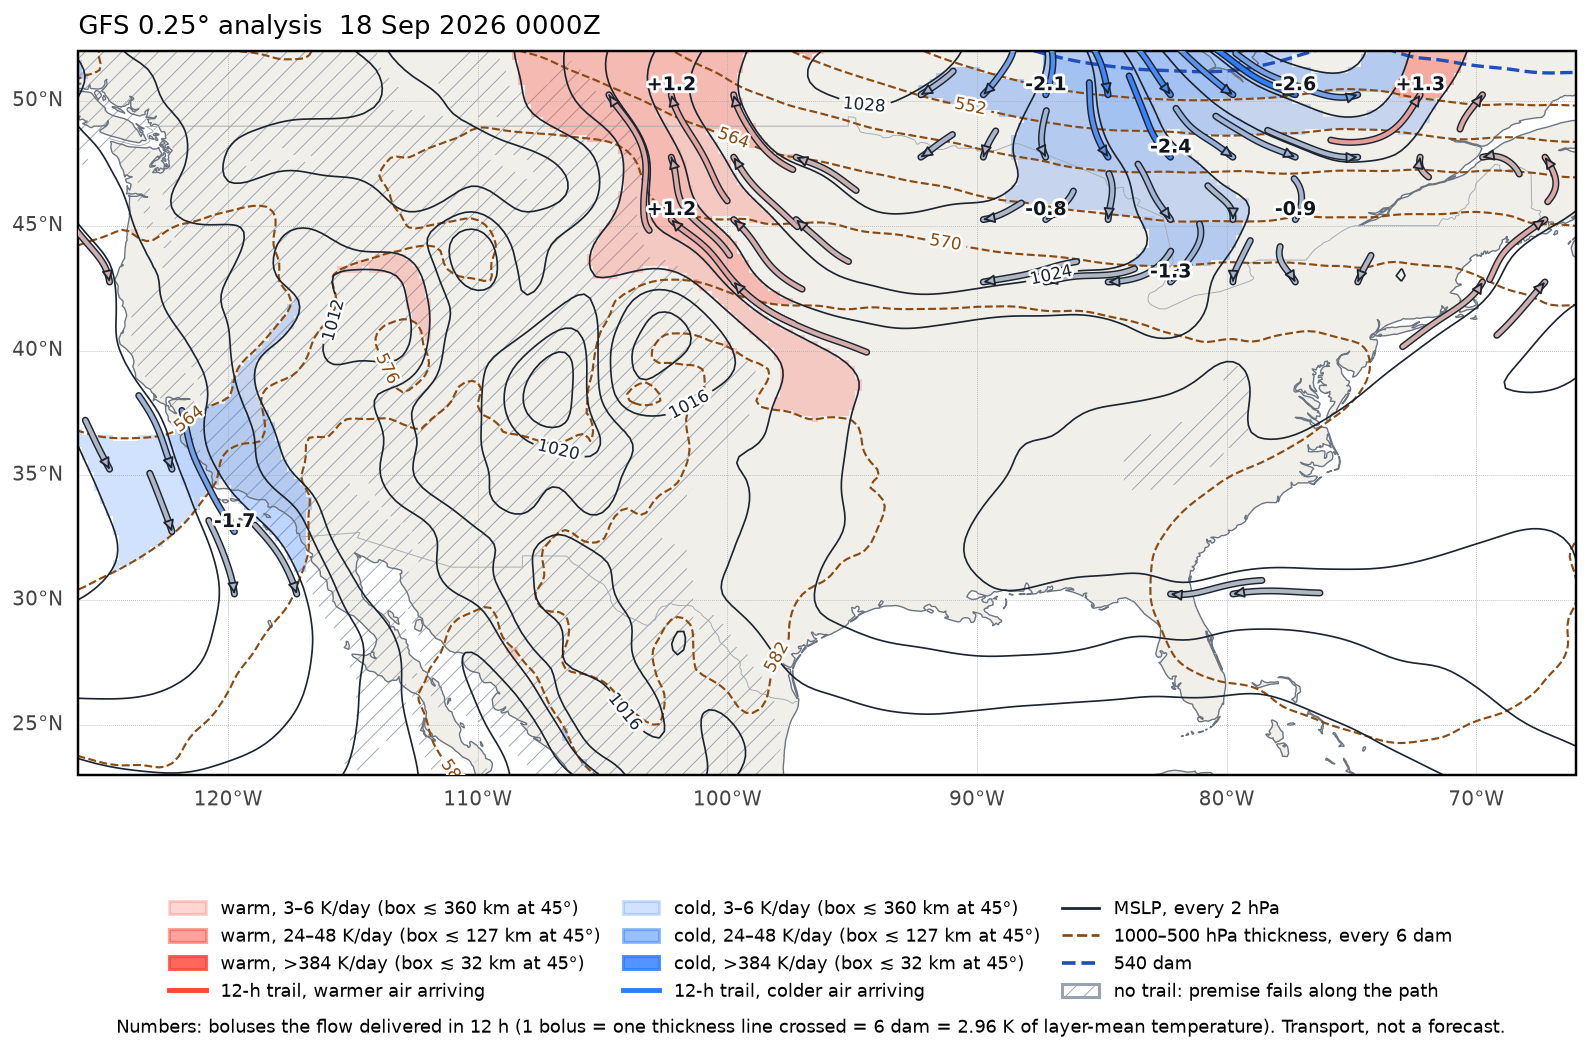
\includegraphics[width=\textwidth]{fig6_transport_conus.png}
\caption{Transport along the channel, continental United States, GFS $0.25^\circ$ analysis valid 18 September 2026 0000Z, the cycle of the first single-cycle verification in \S\ref{sec:verify}. Trails are 12-hour back-trajectories down the isobar channels, colored and labeled by the boluses delivered (blue, colder air arriving; red, warmer); box shading and hatching as in Figures~\ref{fig:conus}--\ref{fig:et}. Cold advection of up to $2.6$ boluses arrives over the Great Lakes behind the front, about one bolus of warm air moves up the High Plains ahead of the next trough, and the intermountain West is hatched throughout for terrain.}
\label{fig:origin}
\end{figure}

\section{Verification}
\label{sec:verify}

The identity was tested against GFS $0.25^\circ$ fields with a harness that compares the box field (\ref{eq:jac}), evaluated pointwise on the chart's own smoothed fields with the tapers on, with the model's advection of the same thickness field by its actual winds. It was run on twelve cycles, the 15th of each month from October 2025 to September 2026, alternating 0000Z and 1200Z, over four scoring windows: the continental United States ($25$--$52^\circ$N, $125$--$67^\circ$W), Europe ($36$--$62^\circ$N, $12^\circ$W--$32^\circ$E), the South Indian Ocean ($28$--$60^\circ$S, $30$--$115^\circ$E), and the South Atlantic ($28$--$60^\circ$S, $50^\circ$W--$15^\circ$E). That is 48 runs across every season in both hemispheres, two windows over land with high terrain and two over open ocean. Scores are $\cos\varphi$-weighted and taken only on points where the premise held. Every entry below is the mean over the 48 runs with the range in parentheses.

Two definitions fix what the numbers mean. The level advection is $-\mathbf{V}_p\cdot\nabla h$, with $\mathbf{V}_p$ the model's full horizontal wind at pressure $p$, not its geostrophic part, and $h$ the same smoothed 1000--500\hPa\ thickness the box field uses; the layer-mean row uses the mean of the winds at 1000, 850, 700, and 500\hPa. Every slope is the least-squares slope of the comparison field regressed on the box field, $\mathrm{cov}(A, y)/\mathrm{var}(A)$, so a slope below one means the box field is the larger of the two.

\paragraph{Fidelity.} Against advection of the thickness by the real wind:

\begin{center}
\begin{tabular}{@{}lcc@{}}
\toprule
Compared against & $r$ & slope \\
\midrule
Full-wind layer-mean advection & 0.95 (0.78--0.99) & 0.83 (0.63--0.99) \\
500\hPa & 0.89 (0.72--0.97) & 0.96 (0.68--1.17) \\
700\hPa & 0.89 (0.64--0.97) & 0.87 (0.64--1.07) \\
850\hPa & 0.91 (0.64--0.98) & 0.91 (0.55--1.11) \\
1000\hPa & 0.78 (0.36--0.93) & 0.58 (0.16--0.94) \\
\bottomrule
\end{tabular}
\end{center}

\noindent The 500\hPa\ row is the clean test of (\ref{eq:split}): there the level-independence of \S2 is exact, so the only difference between the two sides is how far the real 500\hPa\ wind departs from geostrophic, and the slope is 0.96. The 1000\hPa\ row is the friction layer, and it separates the windows as it should: the slope is $0.37$ over the United States and $0.71$ over the South Indian Ocean, where there is less friction and no terrain. The intermediate rows mix two effects, ageostrophy and the turning of the thermal gradient with height, and do not separate them. The layer-mean correlation is $0.98$ and $0.97$ over the two ocean windows and $0.91$ over the United States; the lowest single value, $0.78$, is a weak-gradient February day there. The result is a prediction of the derivation, not a fit, and no run contradicts it.

\paragraph{Advection is not tendency.} The tendency is a centered six-hour difference of the thickness about forecast hour 3 of each cycle, and the advection is evaluated at that hour. Against it, at 42\km\ smoothing, the box field has $r = 0.62$ ($0.11$--$0.89$) and slope $0.50$ ($0.08$--$0.78$); the model's own full-wind advection has $r = 0.62$ and slope $0.57$. Advection overstates the local change by about a factor of two on average, and does so for the model's total advection as much as for the geostrophic part. That is the adiabatic cancellation of \S\ref{sec:temp}, a property of the atmosphere rather than of the technique, and it varies with where and when: the mean slope is $0.35$ over the United States, where a first single-cycle test gave $0.31$, against $0.49$ over Europe, $0.54$ over the South Atlantic, and $0.62$ over the South Indian Ocean. Over land the six-hour thickness change also carries the diurnal cycle, which no advection explains, so the land figures overstate the cancellation by an amount this test does not isolate. In that first cycle the geostrophic field tracked the tendency better than the total advection did. Across the 48 runs it does so in 54\% of them, which is a coin, and no such claim is made.

\paragraph{What it is not.} A kinematic extrapolation of the thickness field by (\ref{eq:jac}), scored against the verifying analysis, has no dependable skill over persistence. The mean skill score is $-0.07$, $-0.35$, and $-0.87$ at 6, 12, and 24 hours (medians $+0.09$, $-0.12$, $-0.37$), and it beats persistence in 58\%, 46\%, and 21\% of the runs. It is worst where the cancellation is strongest, $-0.71$ at six hours over the United States, and marginally positive over the South Indian Ocean ($+0.28$ and $+0.13$ at 6 and 12 hours) before going negative at 24. Pointwise correlation between the box field and model ascent, $-\omega$, at 850, 700, and 500\hPa\ averages $0.10$, $0.12$, and $0.10$ at $0.25^\circ$ and never exceeds $0.30$; for $-\nabla^2 A$ it averages $0.02$. The product is a diagnostic of what the flow is doing to the thermal field now, not a forecast and not an ascent diagnostic.

\section{Consistency checks}
\label{sec:checks}

Two checks are cheap on any grid and should accompany the figures; a third checks the implementation rather than the physics. All three were run on the analysis of Figure~\ref{fig:winter}, 07 September 2026 1200Z, over its frame south of the latitude taper, where the tapered pointwise field has an RMS of $8.6\Kday$.

\paragraph{Thermal-wind cancellation.} Compute $-\mathbf{V}\cdot\nabla h$ with the full layer-mean geostrophic wind $\mathbf{V} = \mathbf{V}_0 + \tfrac12\mathbf{V}_T$ and with $\mathbf{V}_0$ alone. With $\mathbf{V}_T$ taken from the same smoothed $h$ that is being advected, the two agree to round-off: the residual RMS is $5\times10^{-17}$ of the field's RMS and its maximum $9\times10^{-16}$, because the centered-difference Jacobian $J(h,h)$ vanishes term by term, so (\ref{eq:split}) holds for the discrete operator and not only in the continuum. The test with content is the chart's actual recipe, in which the isobars are smoothed at $\sigma = 3.0$ and the heights at $1.5$, so that the thermal wind implied by the two plotted surfaces is not exactly along the plotted thickness lines. There the residual RMS is $5.2\%$ of the field's RMS, the two fields correlate at $0.999$, and the largest pointwise residual is $1.1$ times the field's RMS, at a single tight gradient. That measures the mutual consistency of the chart's two smoothings, not any failure of (\ref{eq:split}).

\paragraph{Interval invariance.} The box rate, quantum over area, is invariant to the intervals only in the limit of small boxes; at finite size it is an area mean over the box, and a finer interval resolves structure a coarser one averages away. Re-rendering against the house $4\hPa$ and $6\dam$, the fraction of the shaded area whose band moves is:

\begin{center}
\begin{tabular}{@{}cccc@{}}
\toprule
$\delta p$ (hPa) & $\delta h$ (dam) & moved $\ge 1$ rung & moved $\ge 2$ rungs \\
\midrule
2 & 6 & 27\% & 4\% \\
8 & 6 & 40\% & 5\% \\
4 & 3 & 44\% & 6\% \\
4 & 12 & 57\% & 14\% \\
2 & 3 & 51\% & 10\% \\
8 & 12 & 66\% & 20\% \\
\bottomrule
\end{tabular}
\end{center}

\noindent A rung is a factor of two in rate, so a one-rung move is the expected cost of a box-mean, and it is common. Two-rung moves are confined to a twentieth of the shaded area when one interval changes by a factor of two and the thickness interval stays at or below the house value. The shaded fraction of the chart itself barely moves between $2$ and $4\hPa$ ($31\%$ against $30\%$). The reading is that the bands are good to a rung, not that they are invariant, and that the $12\dam$ interval is too coarse for the technique on a $0.25^\circ$ analysis.

\paragraph{Box rate against the pointwise field.} The rate assigned to each box should equal the box-mean of the pointwise $A$ from (\ref{eq:jac}). Of 1151 labeled regions on this chart, 438 are whole boxes in the sense of \S\ref{sec:render}. For the 310 whole boxes that are shaded, untapered, and clear of the frame, the ratio of quantum-over-area to the box-mean of $|A|$ has a median of $1.003$ and a 10th-to-90th-percentile range of $0.974$ to $1.044$, and $92\%$ of them land in the same band by either route: (\ref{eq:quantum}) holds on a real grid to a few percent. The 95 partial regions that would otherwise have been shaded, a quarter of the shaded area, are a different matter. Rated at quantum over area they come out a median of 173 times the box-mean of $|A|$, because they are not boxes and do not contain a quantum. That was a labeling error in the first implementation, found by this check, and it is why the renderer now requires all four sides.

\section*{Acknowledgments}

The author first met the technique, and its name, in the weather forecaster course at Keesler Air Force Base and in the Marine Corps follow-on training that succeeds it, and thanks SSgt Matthew Cline, USMC, who taught the latter and made sure it stuck. John Knox (University of Georgia) read a draft and suggested the cold-season case, which is Figure~\ref{fig:winter}. The author declares no competing interests and received no funding for this work.

\section*{Code and data availability}

The renderer described here (constants, box labeling, the whole-box rule, tapers, and shading; \texttt{fb\_boxology.py}), the trajectory operator behind the trails (\texttt{fb\_boxfcst.py}), the verification and consistency harness of \S\S\ref{sec:verify}--\ref{sec:checks} (\texttt{boxology\_verify.py}), the script that made every figure here (\texttt{boxology\_figures.py}), and the archive reader they share (\texttt{fb\_gfsarchive.py}) are part of the FrostByte meteorological product suite and are released with this note at \url{https://github.com/cardboardsinxoverx/boxology} and archived at \url{https://doi.org/10.5281/zenodo.22844862}. They run standalone: the box labeling and shading need only NumPy, SciPy, Matplotlib, and Cartopy, and the harness and figure script add \texttt{requests} and \texttt{cfgrib}; nothing else of the suite is imported except its ETOPO1 reader for the terrain taper, which can be replaced by any elevation array. The exact commands, the per-run results behind every number in \S\S\ref{sec:verify}--\ref{sec:checks}, and the Krovanh track file are included. The governing equations and constants are documented in full, alongside the rest of the suite's physical basis, in the companion technical reference \citep{lane2026}.

All analyses are operational NCEP GFS $0.25^\circ$ fields, 1000 and 500\hPa\ geopotential height and, for the verification, winds and vertical velocity at 1000, 850, 700, and 500\hPa. Every figure and the 48 verification runs were read from the NOAA Open Data Dissemination archive on Amazon Web Services (\url{https://noaa-gfs-bdp-pds.s3.amazonaws.com}, files \path{gfs.YYYYMMDD/HH/atmos/gfs.tHHz.pgrb2.0p25.fFFF}), by byte range from the index files, so any of them can be regenerated. The suite's live products read the same files from the NOMADS grib filter (\url{https://nomads.ncep.noaa.gov/cgi-bin/filter_gfs_0p25.pl}), which keeps about ten days. Elevation is ETOPO1, ice surface (NOAA National Centers for Environmental Information). Krovanh's positions are Japan Meteorological Agency track data as archived by Digital Typhoon, National Institute of Informatics (\url{https://agora.ex.nii.ac.jp/digital-typhoon/}), retrieved 18 September 2026.

\begin{thebibliography}{9}
\setlength{\itemsep}{2pt}

\bibitem[Bjerknes(1898)]{bjerknes1898}
Bjerknes, V., 1898: \"Uber einen hydrodynamischen Fundamentalsatz und seine Anwendung besonders auf die Mechanik der Atmosph\"are und des Weltmeeres. \emph{Kongl. Svenska Vetenskaps-Akad. Handl.}, \textbf{31}, 1--35.

\bibitem[Hart(2003)]{hart2003}
Hart, R. E., 2003: A cyclone phase space derived from thermal wind and thermal asymmetry. \emph{Mon. Wea. Rev.}, \textbf{131}, 585--616.

\bibitem[Holton and Hakim(2013)]{holton2013}
Holton, J. R., and G. J. Hakim, 2013: \emph{An Introduction to Dynamic Meteorology}. 5th ed. Academic Press.

\bibitem[Lackmann(2011)]{lackmann2011}
Lackmann, G., 2011: \emph{Midlatitude Synoptic Meteorology: Dynamics, Analysis, and Forecasting}. American Meteorological Society.

\bibitem[Lane(2026)]{lane2026}
Lane, E. J., 2026: \emph{FrostByte: Mathematical and physical foundations of the product suite}. FrostByte project.

\bibitem[Petterssen(1956)]{petterssen1956}
Petterssen, S., 1956: \emph{Weather Analysis and Forecasting}. Vol. 1, 2nd ed. McGraw-Hill.

\bibitem[Sutcliffe(1947)]{sutcliffe1947}
Sutcliffe, R. C., 1947: A contribution to the problem of development. \emph{Quart. J. Roy. Meteor. Soc.}, \textbf{73}, 370--383.

\end{thebibliography}

\end{document}
